% Use the command \boldeq for the symbolic equals.  You will need to put in the spacing though like $a\ \boldeq \ b $

In this section, we learn about different uses of the equal sign, entering and editing equations, using the blue guidelines, formatting output, highlighting, alignment of equations, and working with units. 

\section{Mathcad: Equations}\label{sec:Mathcad_equations}

There are often many ways to access tools in Mathcad: through a menu at the top of the screen, a toolbar, a right click with the mouse, or a shortcut keystroke.\\

\noindent \large \textsf{\textbf{Entering Text}} \normalsize\\

To enter simple text anywhere on the screen, click at the desired spot (a red plus sign will appear) and do one of the following:\\

$\bullet$ Type $``$ (the region will become a text region).  Then type your text.

$\bullet$ Use the menu: Insert $>$ Text Region

$\bullet$ Start typing text (the region will become a text region after the first word).\\

\noindent \large \textsf{\textbf{Different uses of the equals sign}} \normalsize\\

To enter equations in Mathcad, it is a bit trickier.  There are in fact \underline{FOUR} different ways to use an equals sign (these will be explained soon):\\

$\bullet$ The evaluation equals sign ($=$)

$\bullet$ The assignment equals sign ($:=$) 

$\bullet$ The symbolic equals sign ($\boldeq$) 

$\bullet$ The global equals definition ($\equiv$)\\

%sample inclusion from Mathcad copied to Word, saved as pdf
%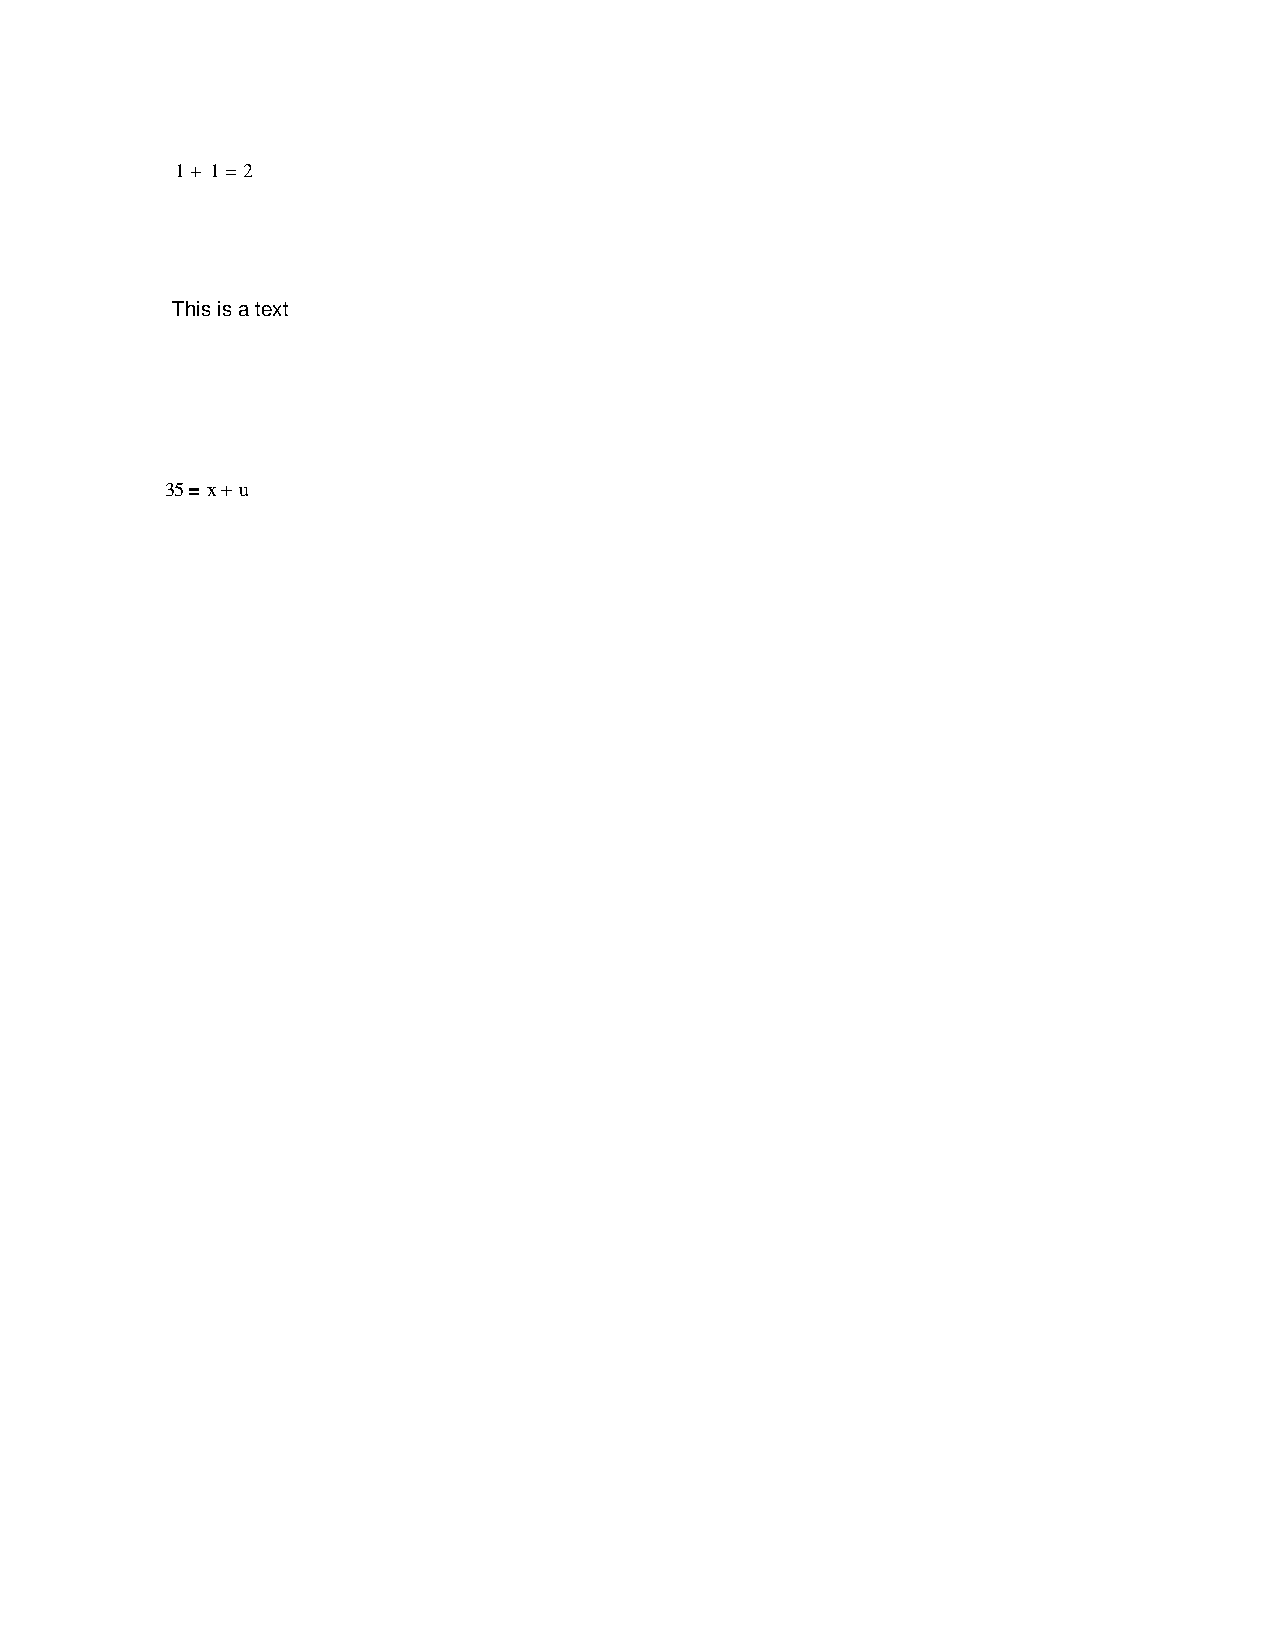
\includegraphics[bb=1in 7.5in 7in 10in]{figures/mathcadsample1.pdf}%bb = llx lly urx ury 
% dimensions of the bounding box are guesses so far.

\index{Mathcad!$=$, Evaluation Equals}
\noindent \large \textsf{\textbf{Evaluation Equals Sign (=)}} \normalsize\\

Mathcad can be used as a simple calulator.  To compute $1+1, 2^{10},$ or $5^{0.5}$, we type these, as one might expect, in the normal way and then type $=$.

\begin{center}
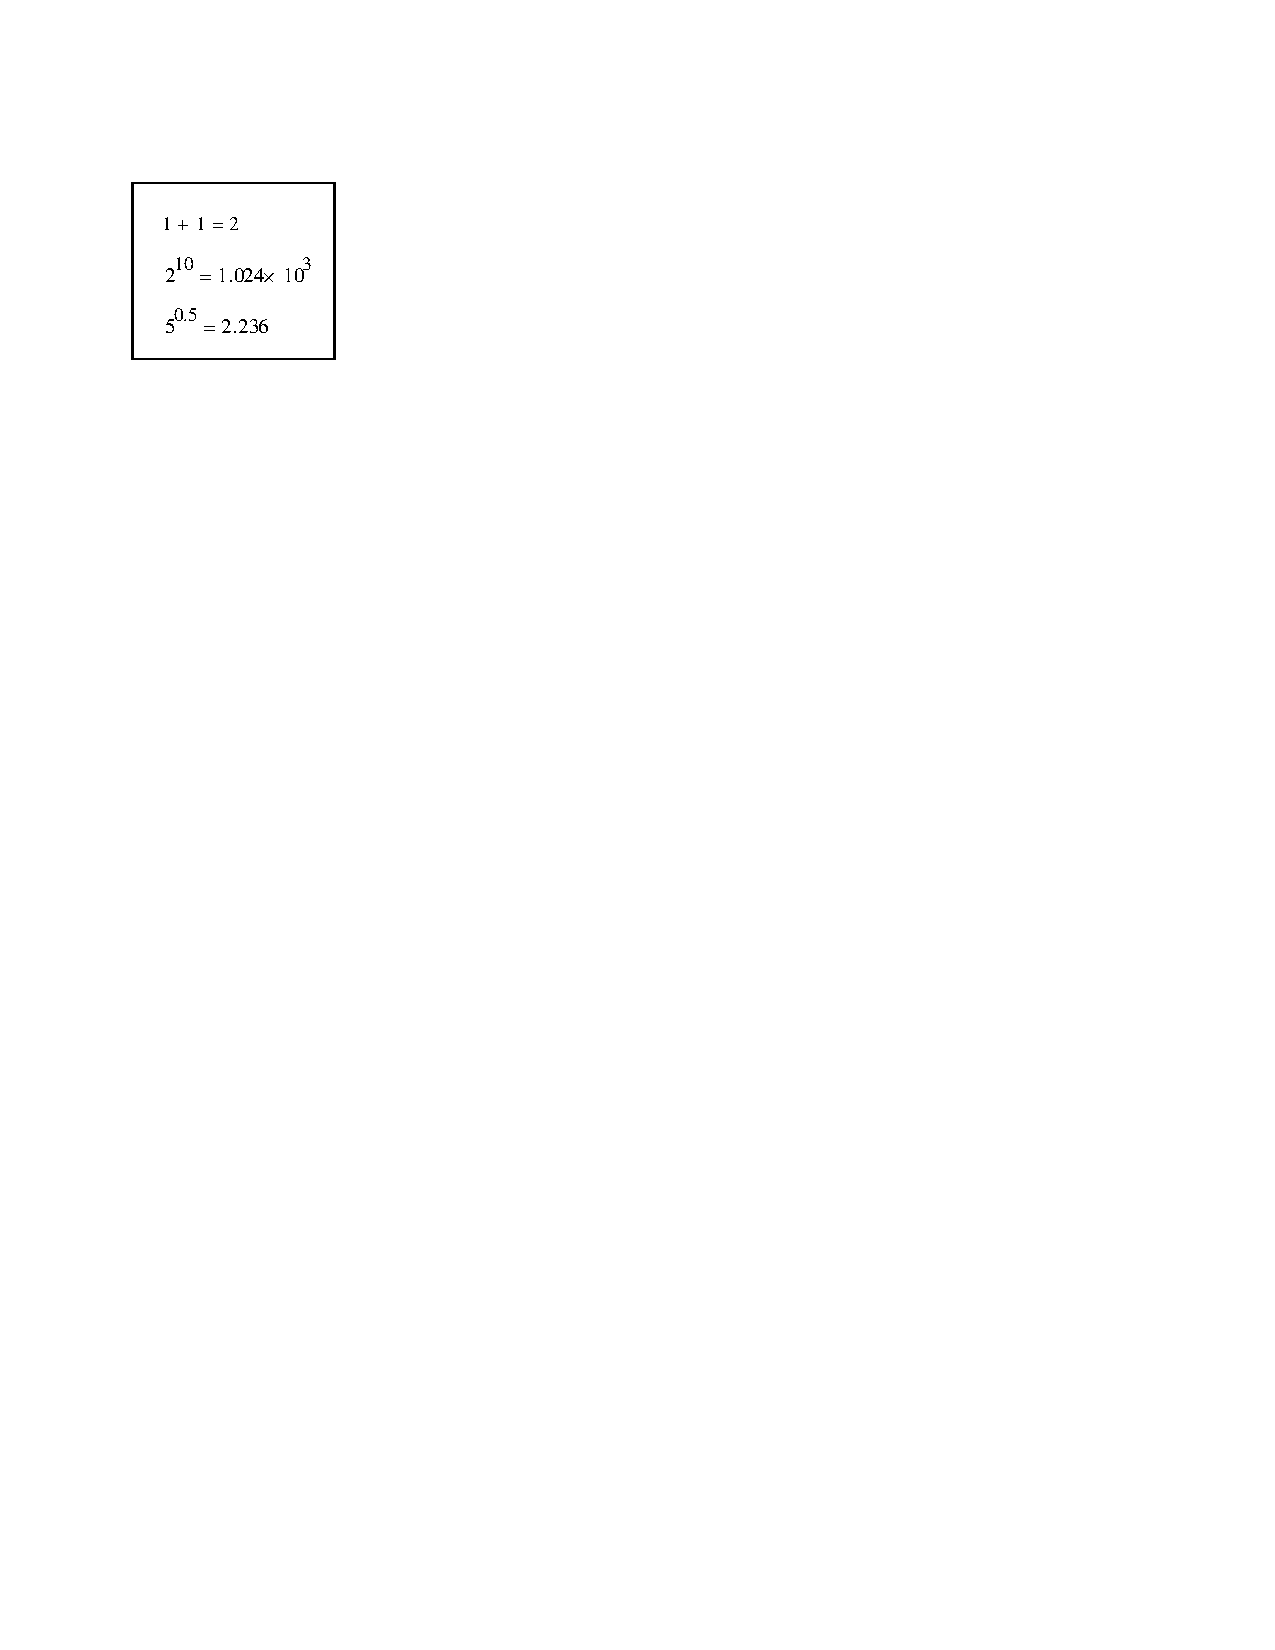
\includegraphics[bb=1in 8.5in 3in 10in]{figures/mathcad_evaluation_equals.pdf} %Mathcad copied to Word, saved as pdf, guess bounding box size
\end{center}

For a few more advanced computations, we can try $\cos(\pi), \sin(90^\circ), \sqrt{5},$ and  $\ln\left(\displaystyle \frac{1}{2}\right).$
\begin{center}
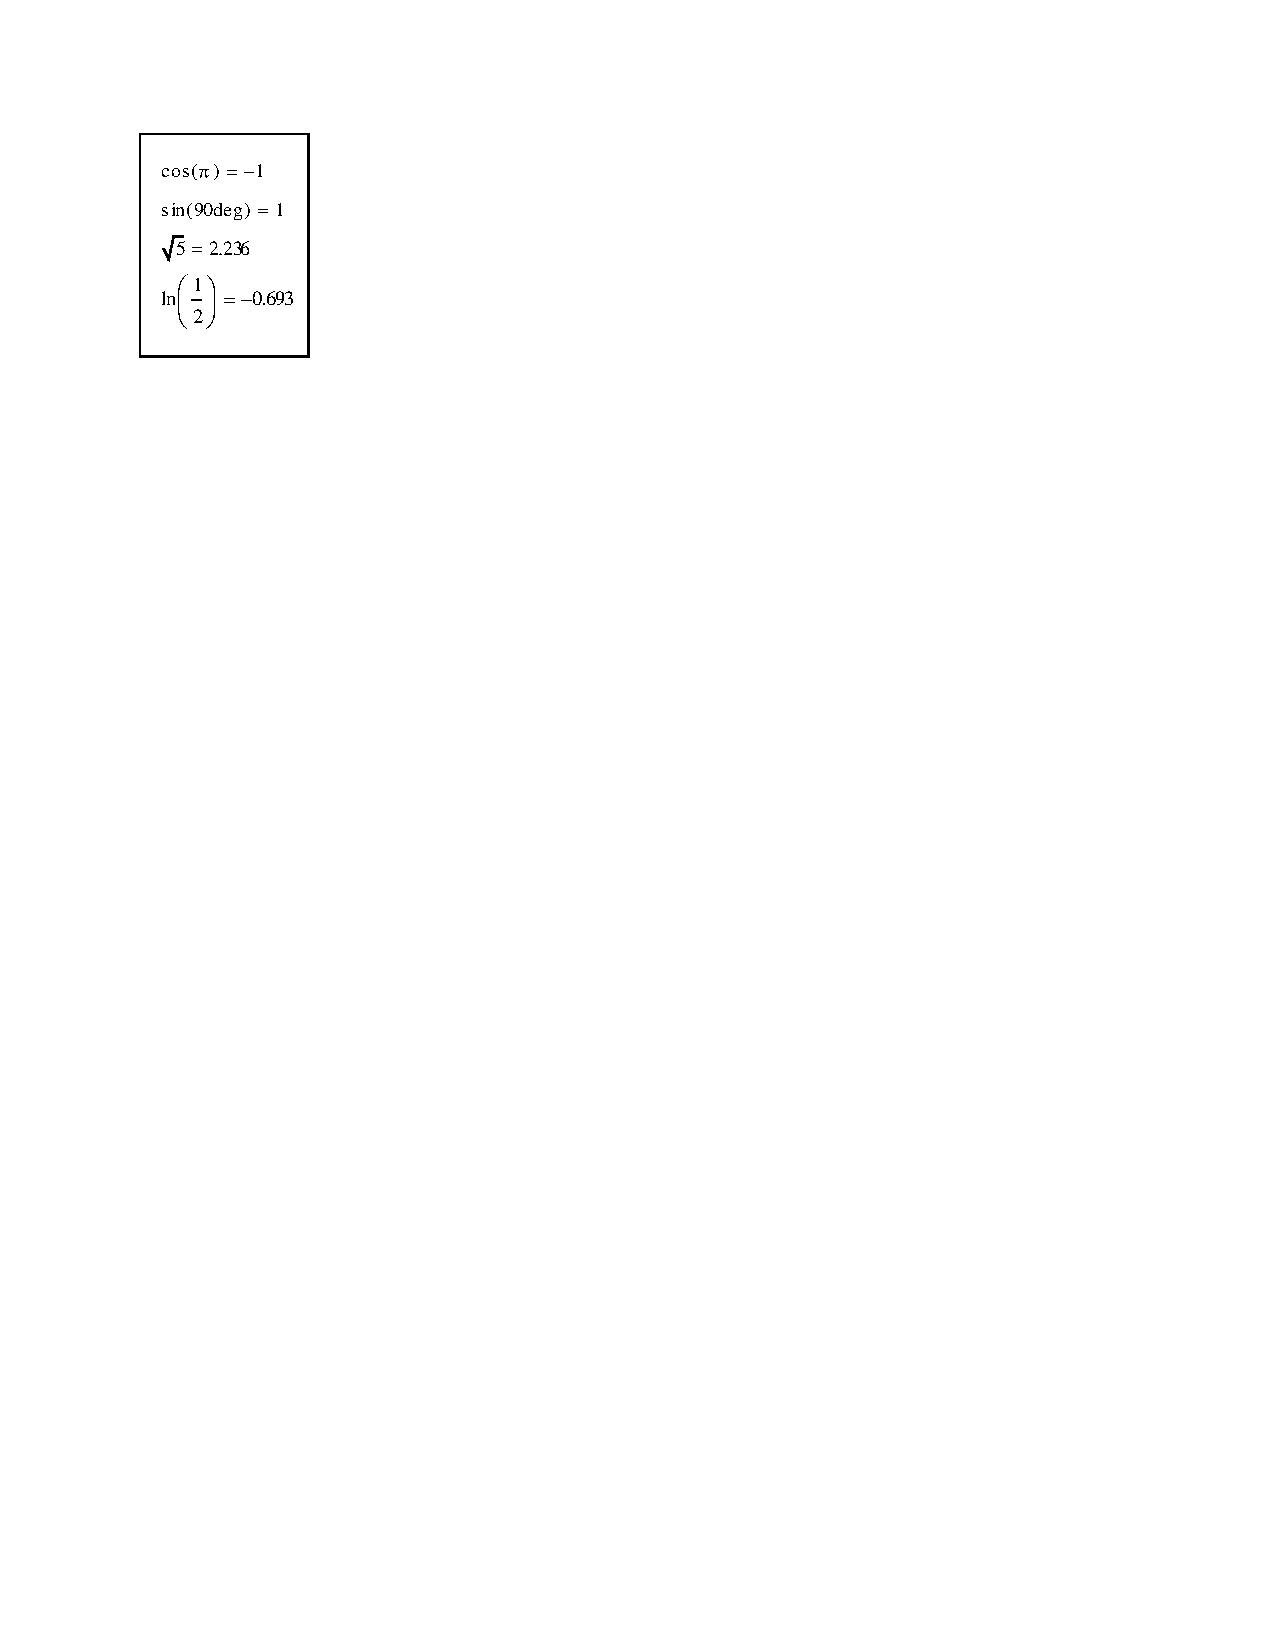
\includegraphics[bb=1in 8.5in 3in 10in]{figures/mathcad_evaluation_equals2.pdf} %Mathcad copied to Word, saved as pdf, guess bounding box size
\end{center}

Creating the symbols in these calculations can be done in many ways!  The trigonometric and natural logarithm are simply typed in as sin, cos and ln.
The symbol for pi can be created from the Greek toolbar, or with the shortcut key ctrl+shift+p (or type p followed by ctrl+g).  Note that the default is radian mode for the trig functions, but if you want degrees, type the word deg inside the trig function (just as it appears).  To get a fraction, type 1, backslash and 2 (the format of the fraction and size of the parentheses are automatically done by Mathcad).  To get the square root symbol, use the calculator toolbar (or shortcut key $\backslash$).

We especially encourage the reader to explore the toolbars, menus, keyboard shortcuts, mouse clicks, help files, etc.  That's how we learned a lot of Mathcad's functionality.  Also, if there is something that you can't figure out, try your favorite internet search engine.  We do.\\

\newpage

\index{Mathcad!$:=,$ Assignment Equals}
\noindent \large \textsf{\textbf{Assignment Equals Sign (:=)}} \normalsize\\

It is often useful to assign values to variables that can be used later.  This is done with the assignment equals sign, created not by using the = key, but by typing a colon (:).

For example, suppose we wanted to find the area of a circle of radius $5$ meters.  We could of course do the calculation ``pi r squared'' but we will instead store the value $5m$ in the variable {\bf radius} and then compute and store the area in the variable {\bf Area}.  Make sure to type a colon instead of = in order to get the symbol :=.

\begin{center}
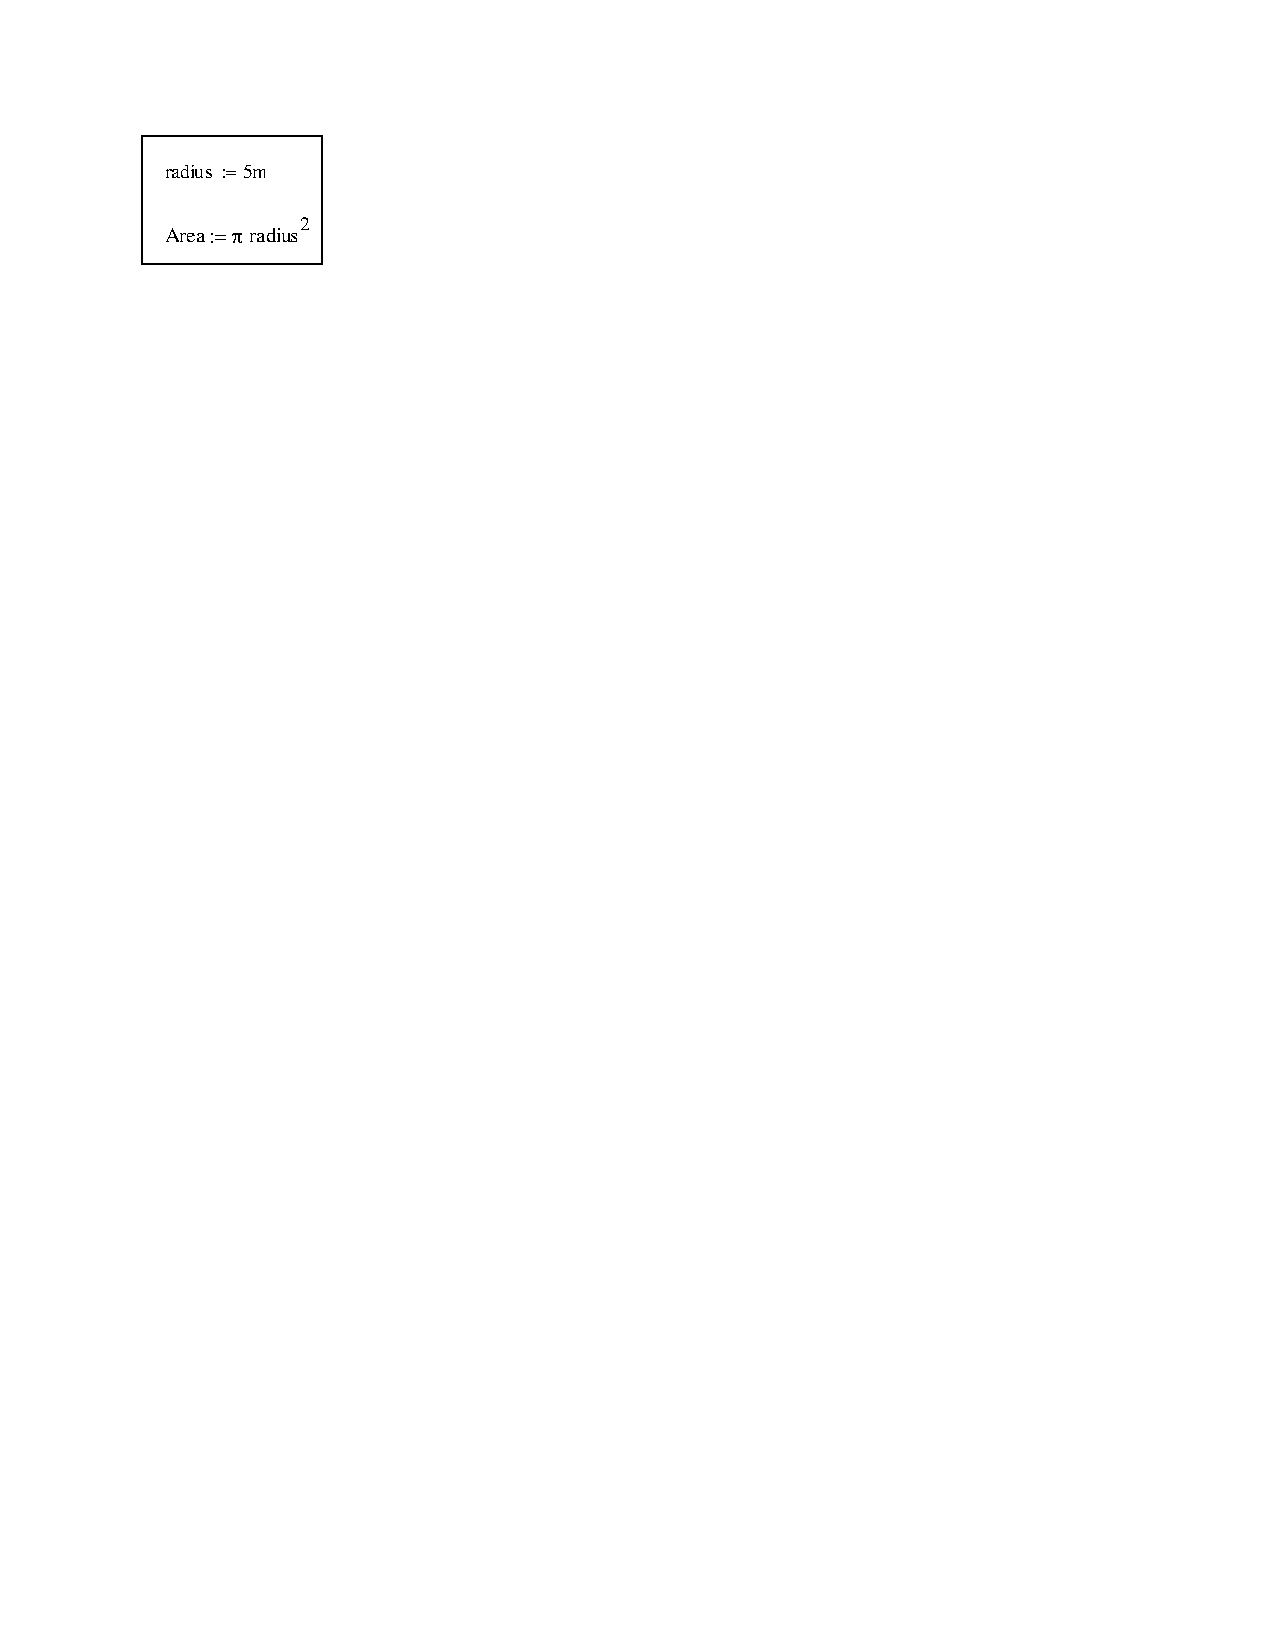
\includegraphics[bb=1in 9.25in 3in 10.2in]{figures/mathcad_assignment_equals.pdf} %Mathcad copied to Word, saved as pdf, guess bounding box size
\end{center}

Note that with the assignment equals, you don't see the actual value of {\bf Area}.  To see the actual value, you need to either put in an additional line

\begin{center}
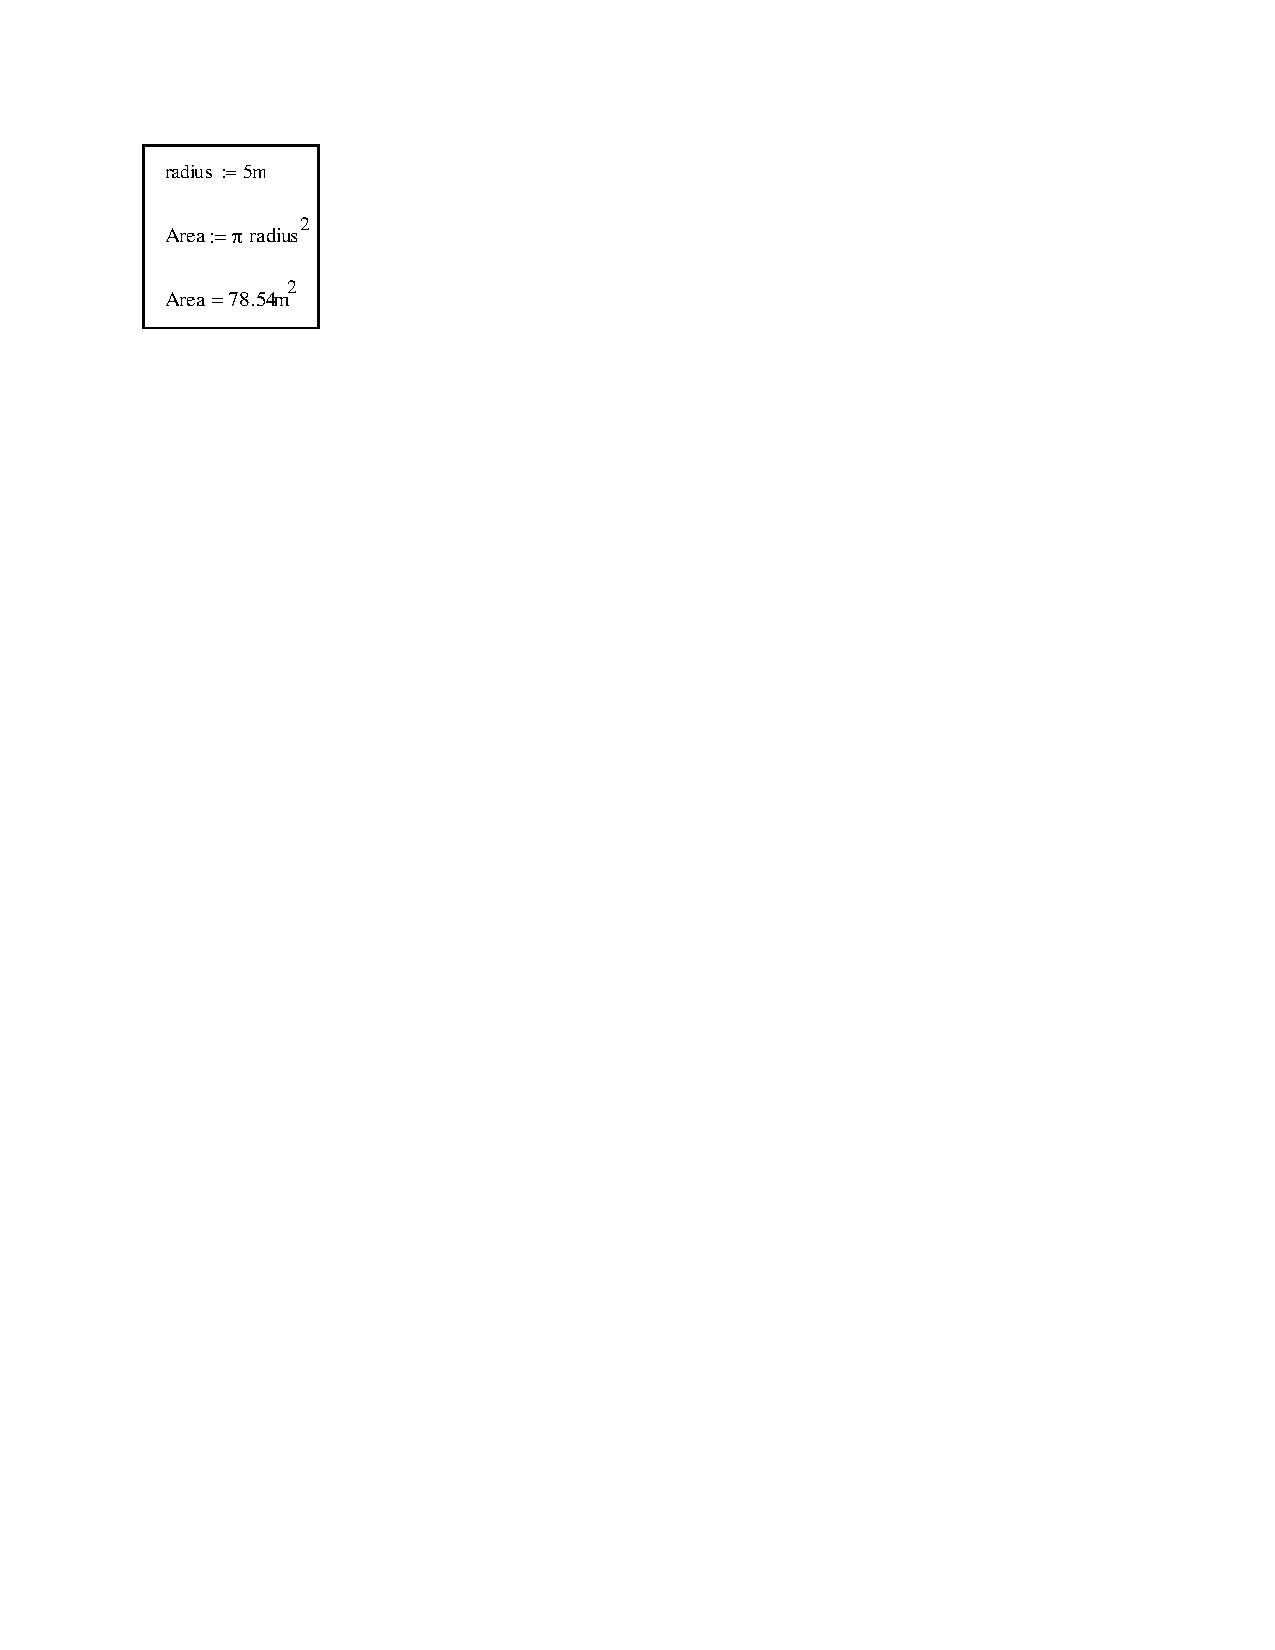
\includegraphics[bb=1in 8.5in 3in 10.2in]{figures/mathcad_assignment_equals2.pdf} %Mathcad copied to Word, saved as pdf, guess bounding box size
\end{center}

(where the second equation with the variable {\bf Area} does use the = sign) or type an additional equals sign ($=$) at the end of the line defining {\bf Area}

\begin{center}
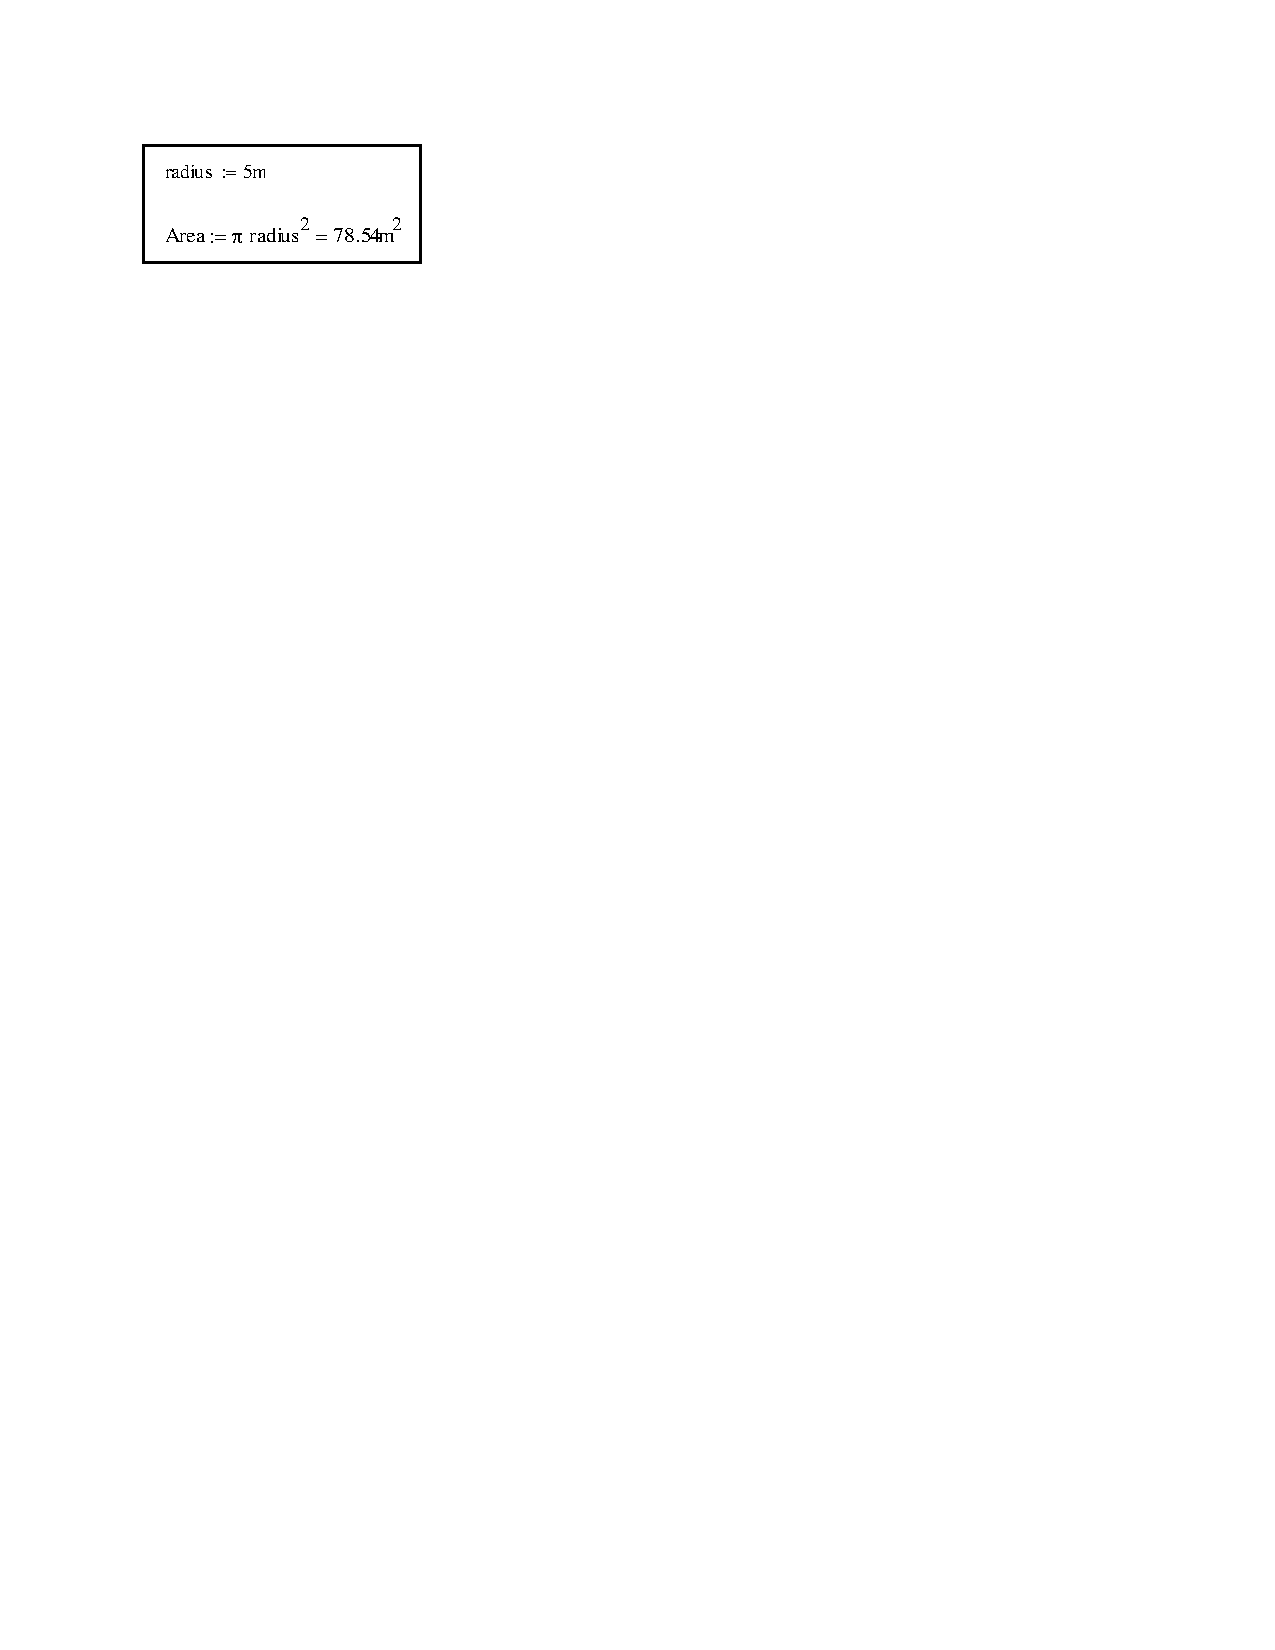
\includegraphics[bb=1in 8.5in 3in 10.2in]{figures/mathcad_assignment_equals3.pdf} %Mathcad copied to Word, saved as pdf, guess bounding box size
\end{center}

\index{Mathcad!${\bf =}$, Symbolic Equals}
\noindent \large \textsf{\textbf{Symbolic Equals Sign ($\raisebox{1pt}{\rule{9pt}{1.5pt}}\hskip-9pt\raisebox{3.5pt}{\rule{9pt}{1.5pt}}$)}} \normalsize\\

The symbolic equals sign (an equals sign appearing in bold font) is used in setting up an equation without actually providing any values for the variables.  For example, in computing the area of a circle, we may not necessarily know the value of the radius, but want to use the equation ``A equals pi r squared.''  If we try to enter this with the assignment equals (without providing the radius value), we get an error (the variable {\bf radius} is in red).

\begin{center}

\includegraphics[bb=1in 9.5in 3in 10.2in]{figures/mathcad_assignment_equals_error.pdf} %Mathcad copied to Word, saved as pdf, guess bounding box size
\end{center}

To fix this, we use the symbolic equals sign (a bold equals sign) by typing Ctrl + =.

\begin{center}

\includegraphics[bb=1in 9.5in 3in 10.2in]{figures/mathcad_assignment_equals_error_fixed.pdf} %Mathcad copied to Word, saved as pdf, guess bounding box size
\end{center}

One reason for using the symbolic equals is that you might want to later solve (symbolically) for the radius in terms of the area.  We will show how to do this and give more reasons why you might want to use the symbolic equals sign in later sections.   \\

\index{Mathcad!$\equiv$, Global Equals}
\noindent \large \textsf{\textbf{Global Equals Definition ($\equiv$)}} \normalsize\\

Consider the following example:

\begin{center}
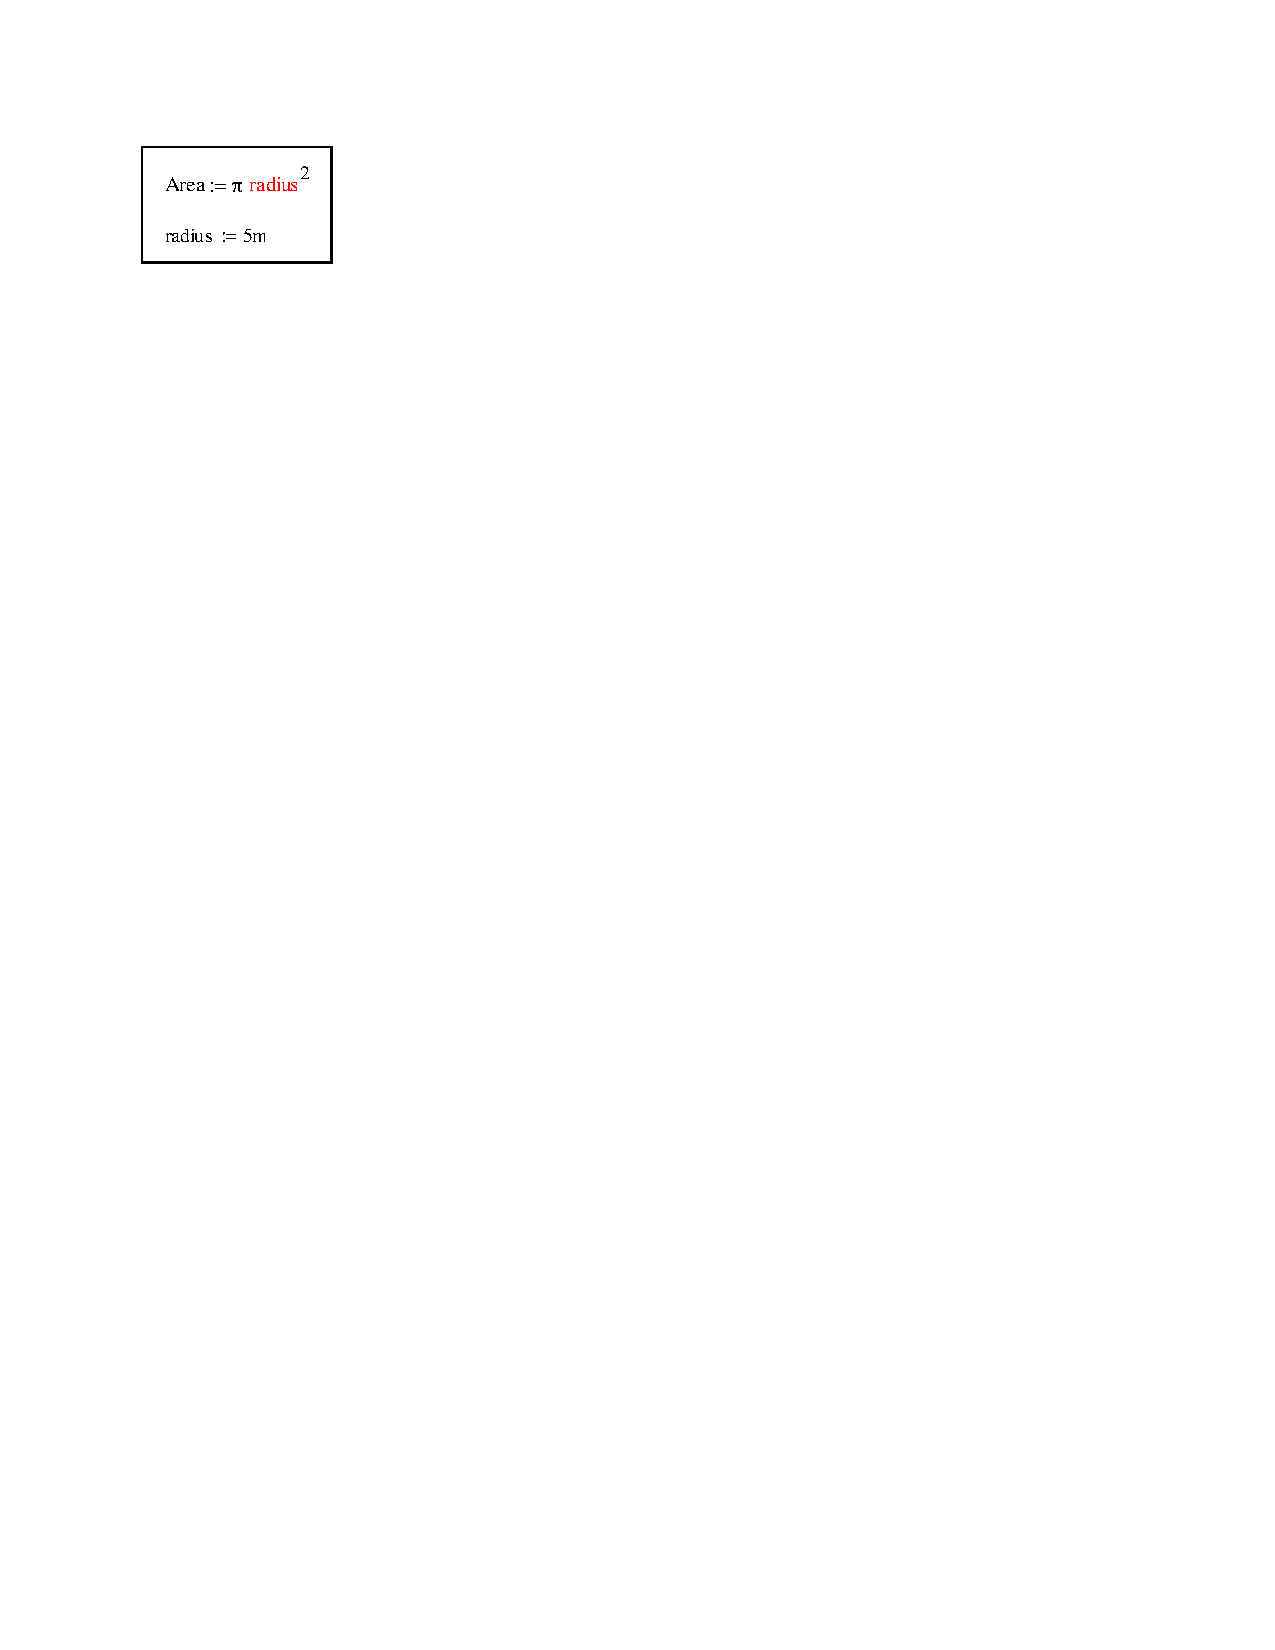
\includegraphics[bb=1in 9in 3in 10.2in]{figures/mathcad_order_of_computation1.pdf} %Mathcad copied to Word, saved as pdf, guess bounding box size
\end{center}

Why is the word {\bf radius} in red?  All of the parts of the computation are present, but for Mathcad, this is not enough.  The order of the computations is important (as we will discuss further).  Mathcad computations have the order ``left to right, top to bottom'' meaning that any variable used in a calculation must be defined previously (either higher up on the page, or to the left on the page).  There is one exception to this rule - the global equals definition.  The global equals definition is created using the tilde ($\sim$) symbol.  A variable that is defined with the global equals definition can be used in any other equation, regardless of its location on the page.  

\begin{center}
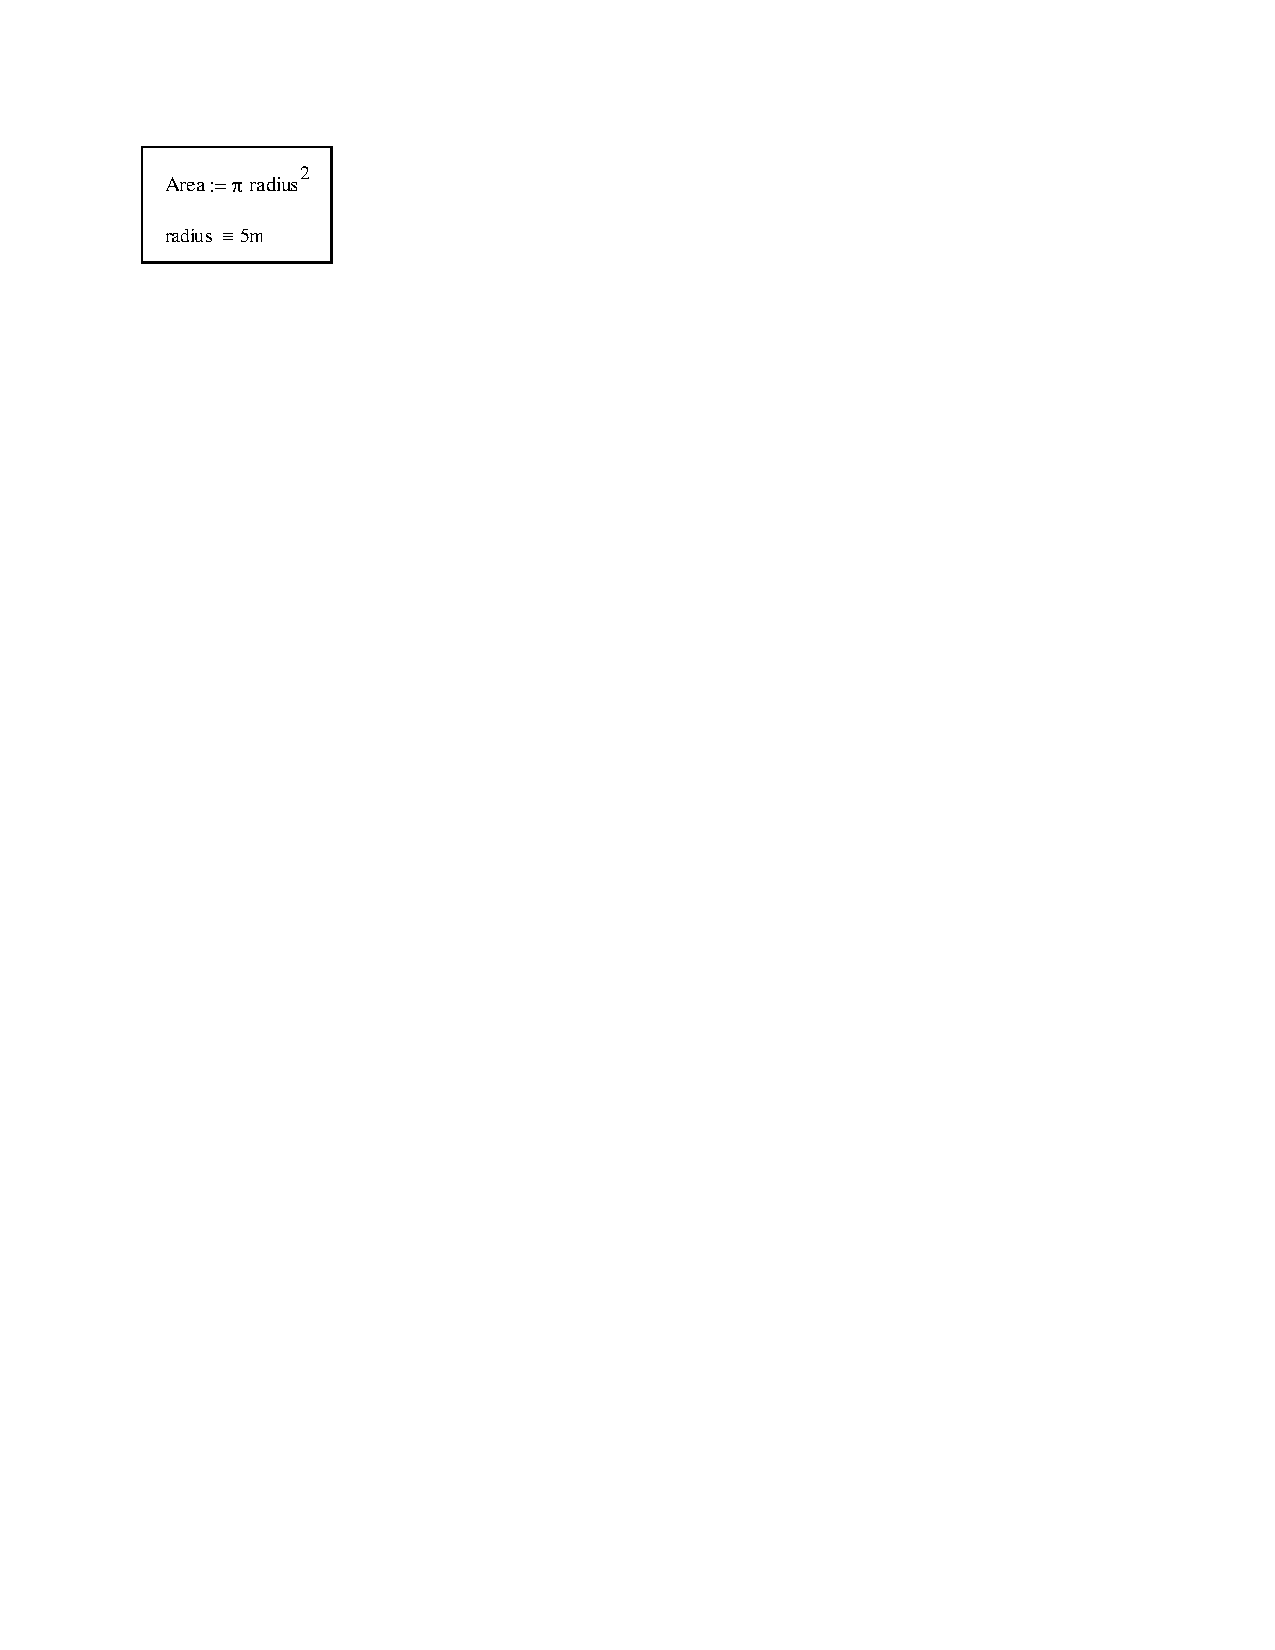
\includegraphics[bb=1in 9in 3in 10.2in]{figures/mathcad_global_definition.pdf} %Mathcad copied to Word, saved as pdf, guess bounding box size
\end{center}

Also, if a variable is defined globally, that does not mean that it will override another definition of the same variable, for example consider

\begin{center}
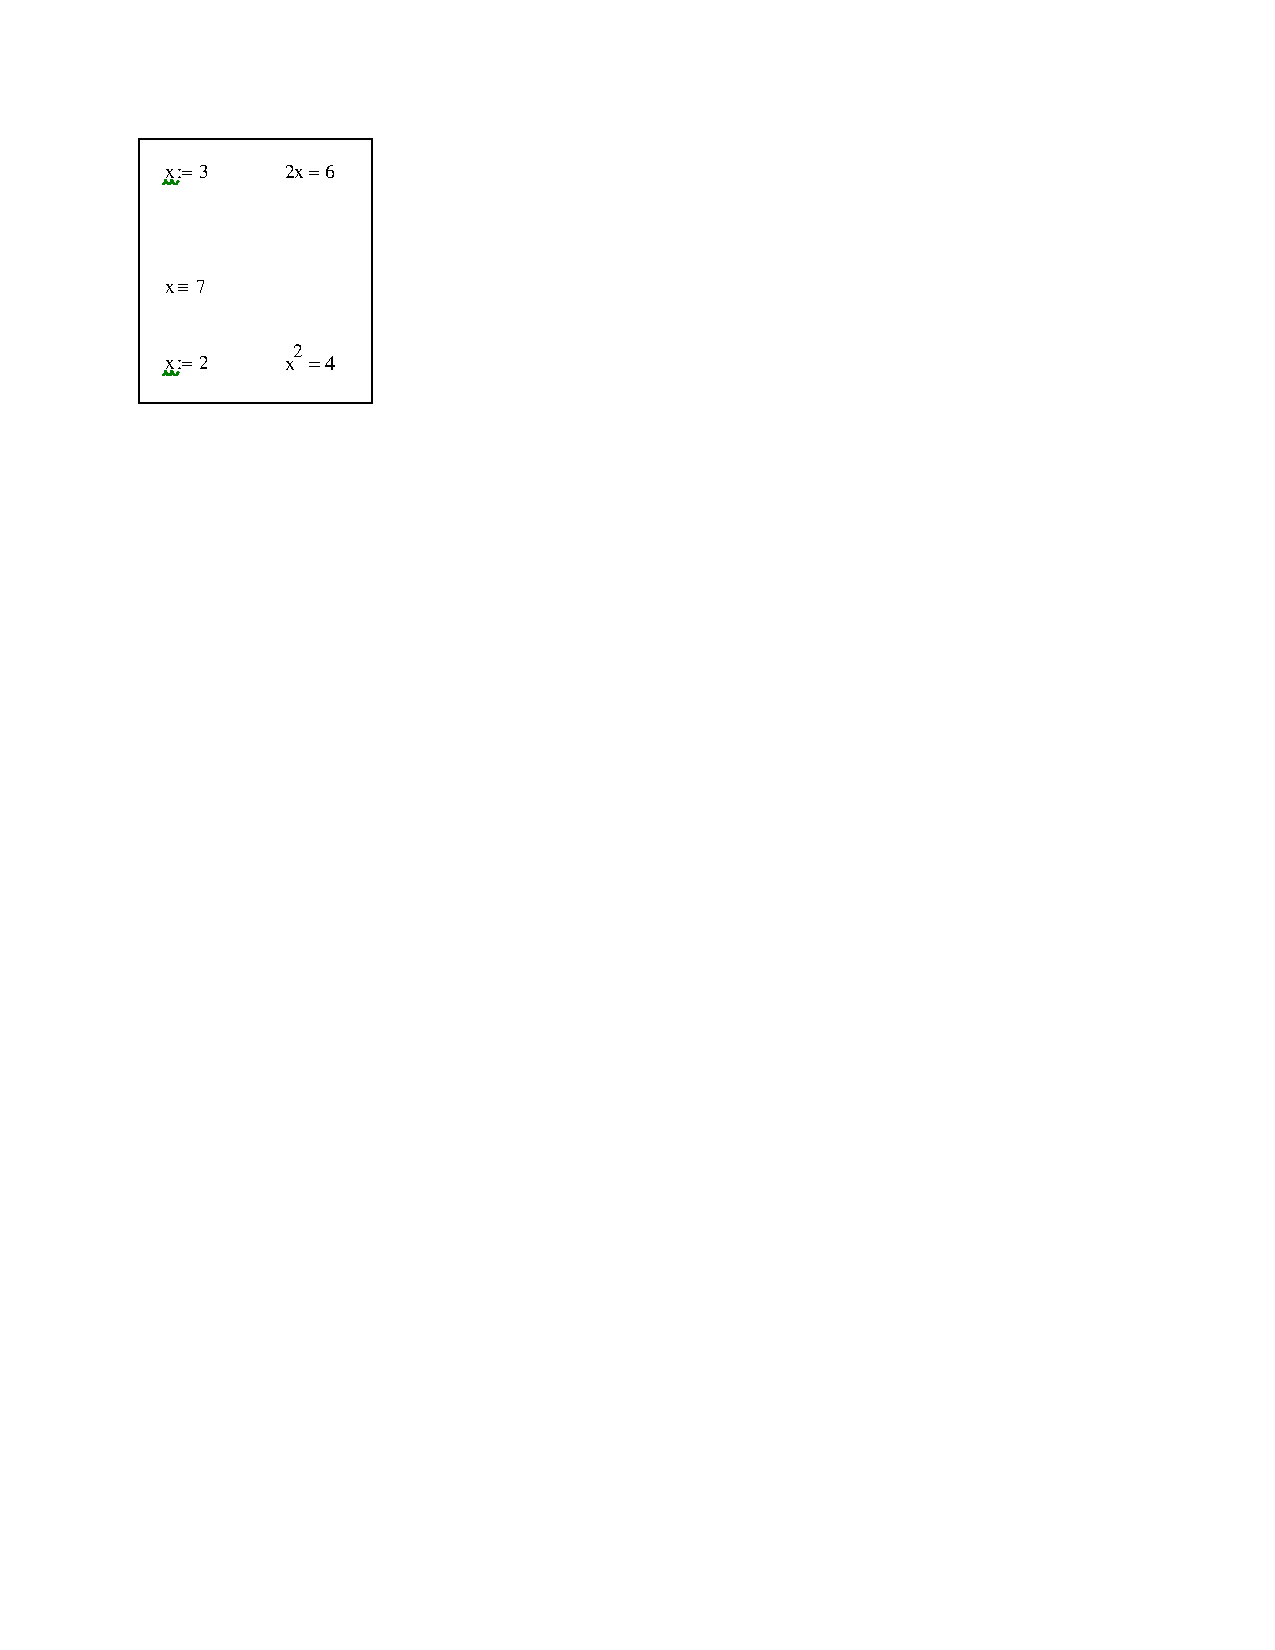
\includegraphics[bb=1in 8in 3in 10.2in]{figures/mathcad_global_definition2.pdf} %Mathcad copied to Word, saved as pdf, guess bounding box size
\end{center}

Here we see that even though $x$ is globally defined to be 7, the top line computation of $2x$ is using $x$ equal to 3 and the bottom line computation of $x^2$ is using $x$ equal to 2.

We strongly suggest \underline{against} using the global equals definition.  Finding errors in equations can be difficult enough without having to worry about possible miscalculations due to a globally defined variable.  
\keyidea{idea:variablenames}{\textbf{Variable Names}\\

In deciding on variable names, consider the following:\\

$\bullet$ Variable names cannot begin with a number. \\

$\bullet$ Use descriptive names such as ``Area'' instead of simply $A$\\

$\bullet$ Try not to use variable names for predefined Mathcad units, like $m$ (meter), $c$ (speed of light), $K$ (degrees Kelvin), etc.  If you try to do so, the variable will be marked with a green squiggly line as a reminder.
}

\section{Mathcad: Editing Equations}\label{sec:Mathcad_editing_equations}

Once an equation is entered, editing it can be tricky.  We recommend first reading the help file under\\ 
\\
Contents $>$ Getting Started $>$ Entering and Evaluating Expressions $>$ Editing an Expression.\\

Here we give a few pointers, but also suggest plenty practice and trial-and-error.\\

\noindent \large \textsf{\textbf{Blue Guidelines}} \normalsize\\

As you type, you should notice a pair of blue lines appear and change size as you enter the expression, one as an underline and one as a vertical line.  This pair of guidelines indicates the insertion point if you were to type something new.  In order to move the blue guidelines to the desired spot you can try the following\\

$\bullet$ Using the \textbf{spacebar}\\

Each time the spacebar is depressed, the blue guidelines increase in length and enclose more of the equation for editing.
Try it.\\

$\bullet$ Using the \textbf{arrow keys}\\

You can scroll through an equation using the left and right arrow keys.  With the up and down arrow keys, you can move between exponents and subscripts. Give it a shot.\\

$\bullet$ Using the \textbf{insert key}\\

Using the insert key, you can move the vertical blue guideline to the opposite side of the horizontal blue guideline. Once, again, you'll figure it out by trying it.\\

\noindent \large \textsf{\textbf{Using the mouse}} \normalsize\\

You can of course use the mouse to click within an equation or to move selected equation blocks.  

To edit within an equation, click at the desired location in the equation.  If you want to select a variable name, try double clicking on the variable name, or highlighting it with the usual click-and-drag.

To select multiple equations into a block that can be moved or aligned, click and hold at a location outside the equation and drag the dotted box that appears to include the desired equations.  Once the mouse button is released, the selected equations can be moved by putting the mouse cursor over one of the selected boxes (a small hand should appear), then click and move the entire block to the desired location.  

To align a selected block of equations, do one of the following:\\

$\bullet$ Use the menu: Format $>$ Align Regions $>$ (either Across or Down)

\index{Mathcad!Aligning Regions}
$\bullet$ Click on the align Across or align Down button (as pictured).

\vspace{.25in}
\hspace{-.5in}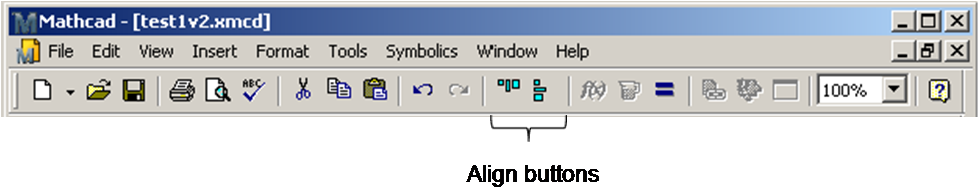
\includegraphics[scale=.8]{figures/mathcad_layout_png2.png} %Mathcad screen shot copied to PP, saved as png file
\vspace{.25in}

\noindent \large \textsf{\textbf{Other Customization of Equation Blocks}} \normalsize\\

One of Mathcad's strengths is the ability of the user to make the work simply look nice.  Combining text and equations along with graphs is easy to do.  In addition, you can customize your equations in a number of ways\\

\index{Mathcad!Highlighting Regions}
$\bullet$ Highlighting the equation \\

This is useful to make parts of the sheet stand out.  If you right click on an equation, you can select Properties.  From there, you can select ``Highlight Region'' (and select a color) or ``Show Border'' (around the equation).\\

\index{Mathcad!Formatting Results}
$\bullet$ Formatting the result \\
  
Under the menu Format $>$ Result, you can set the number of decimal places, change the ``Number format'' (Decimal, Scientific, Engineering, etc.), ``Display Options'' (useful for tables and matrices) and customize how units are shown in ``Unit Display.''  You can also double click any \underline{evaluated} equation to get this dialog box.

\index{Mathcad!Units}
\section{Mathcad: Units}\label{sec:Mathcad_units}

A very powerful part of Mathcad comes from its ability to handle units and unit conversions.  When entering an equation, you can access the complete set of units under the menu at Insert $>$ Units

\vspace{.35in}
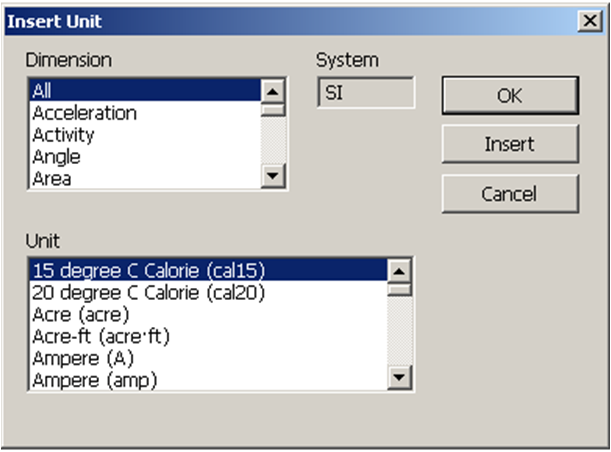
\includegraphics[scale=.8]{figures/mathcad_unit_box.png} %Mathcad screen shot copied to PP, saved as png file
\vspace{.25in}

\noindent or if you know the name of the unit, you can just type it in:


\begin{center}
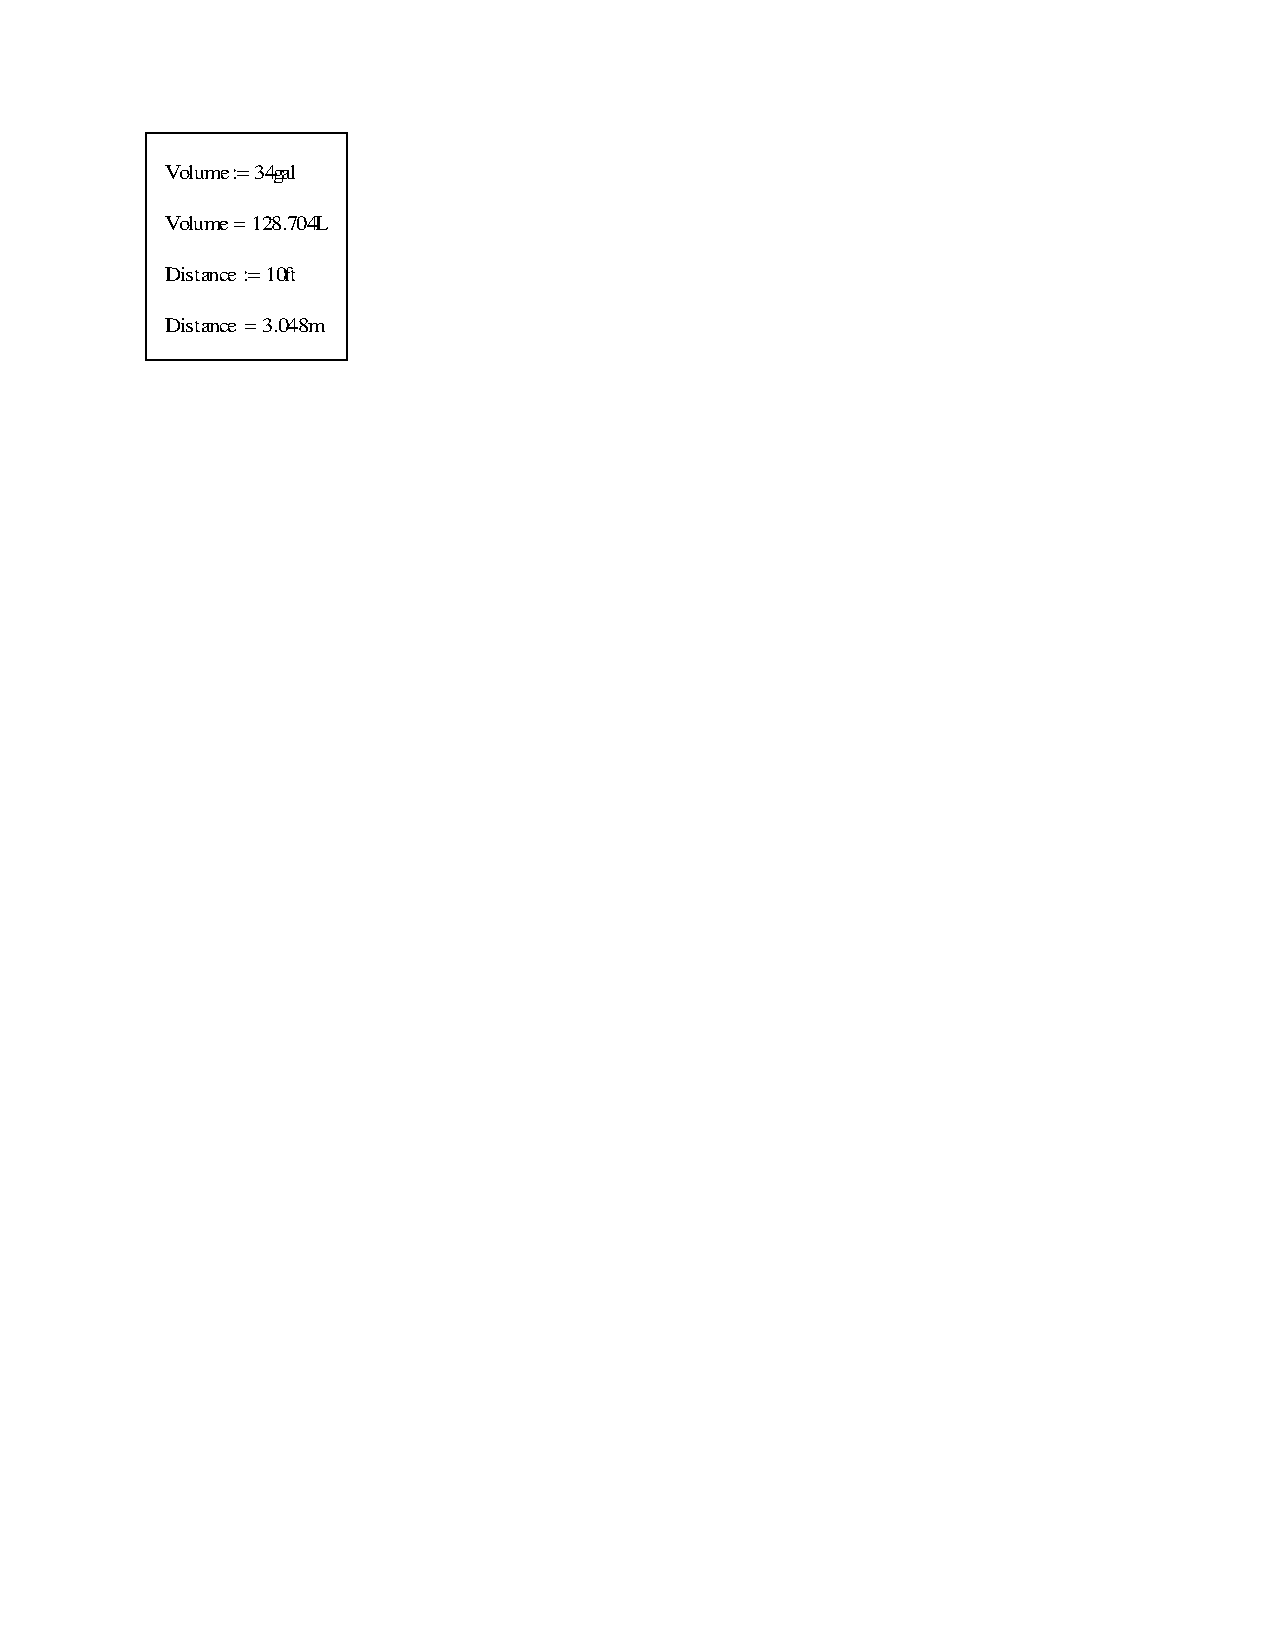
\includegraphics[bb=1in 8.5in 3in 10.25in]{figures/mathcad_units.pdf} %Mathcad copied to Word, saved as pdf, guess bounding box size
\end{center}

%%\begin{center}
%%%{\fontfamily{phv}\selectfont Helvetica looks like this}
%%{\fontfamily{ptm}\selectfont Volume $:=$ 34 gal}\\
%%{\fontfamily{@times@new@roman}\selectfont Volume $=$ 128.704 L}\\
%%{\fontfamily{@times@new@roman}\selectfont Distance $:=$ 10 ft}\\
%%{\fontfamily{@times@new@roman}\selectfont Distance $=$ 3.048 m}\\
%%\end{center}

In this example, we entered the first and third lines exactly as they look, using the colon to make the assignment equals sign $:=$ and typing the letters ``gal'' and ``ft''.  In the second and fourth equations, we used the evaluation equals sign $=$ to calculate.  Note that Mathcad automatically calculates using metric units as a default.

To keep an expression with a specific unit, consider the following example where we want the final answer in feet.  We want to calculate the distance travelled by an object moving at 10 feet per second for 15 minutes. We enter the corresponding variables using the assignment equals in defining \textbf{Velocity}, \textbf{Time} and \textbf{Distance}.  But, in the fourth line, when we use the evaluation equals, Mathcad automatically converts \textbf{Distance} to meters.  To adjust this, first, click at the end of the line where \textbf{Distance} is computed. A small black box appears that we select...


\begin{center}
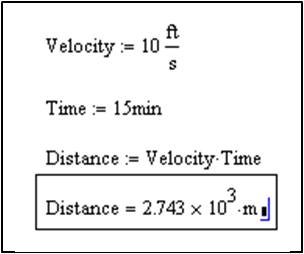
\includegraphics[scale=.85]{figures/mathcad_unit2.png} %Mathcad screen shot copied to PP, saved as png file
\end{center}

... type ft in the box:


\begin{center}
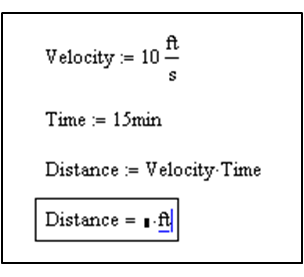
\includegraphics[scale=.85]{figures/mathcad_unit3.png} %Mathcad screen shot copied to PP, saved as png file
\end{center}

... and hit return:


\begin{center}
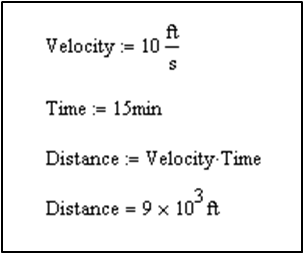
\includegraphics[scale=.85]{figures/mathcad_unit4.png} %Mathcad screen shot copied to PP, saved as png file
\end{center}


%Now, on to the exercises...
%\begin{center}
%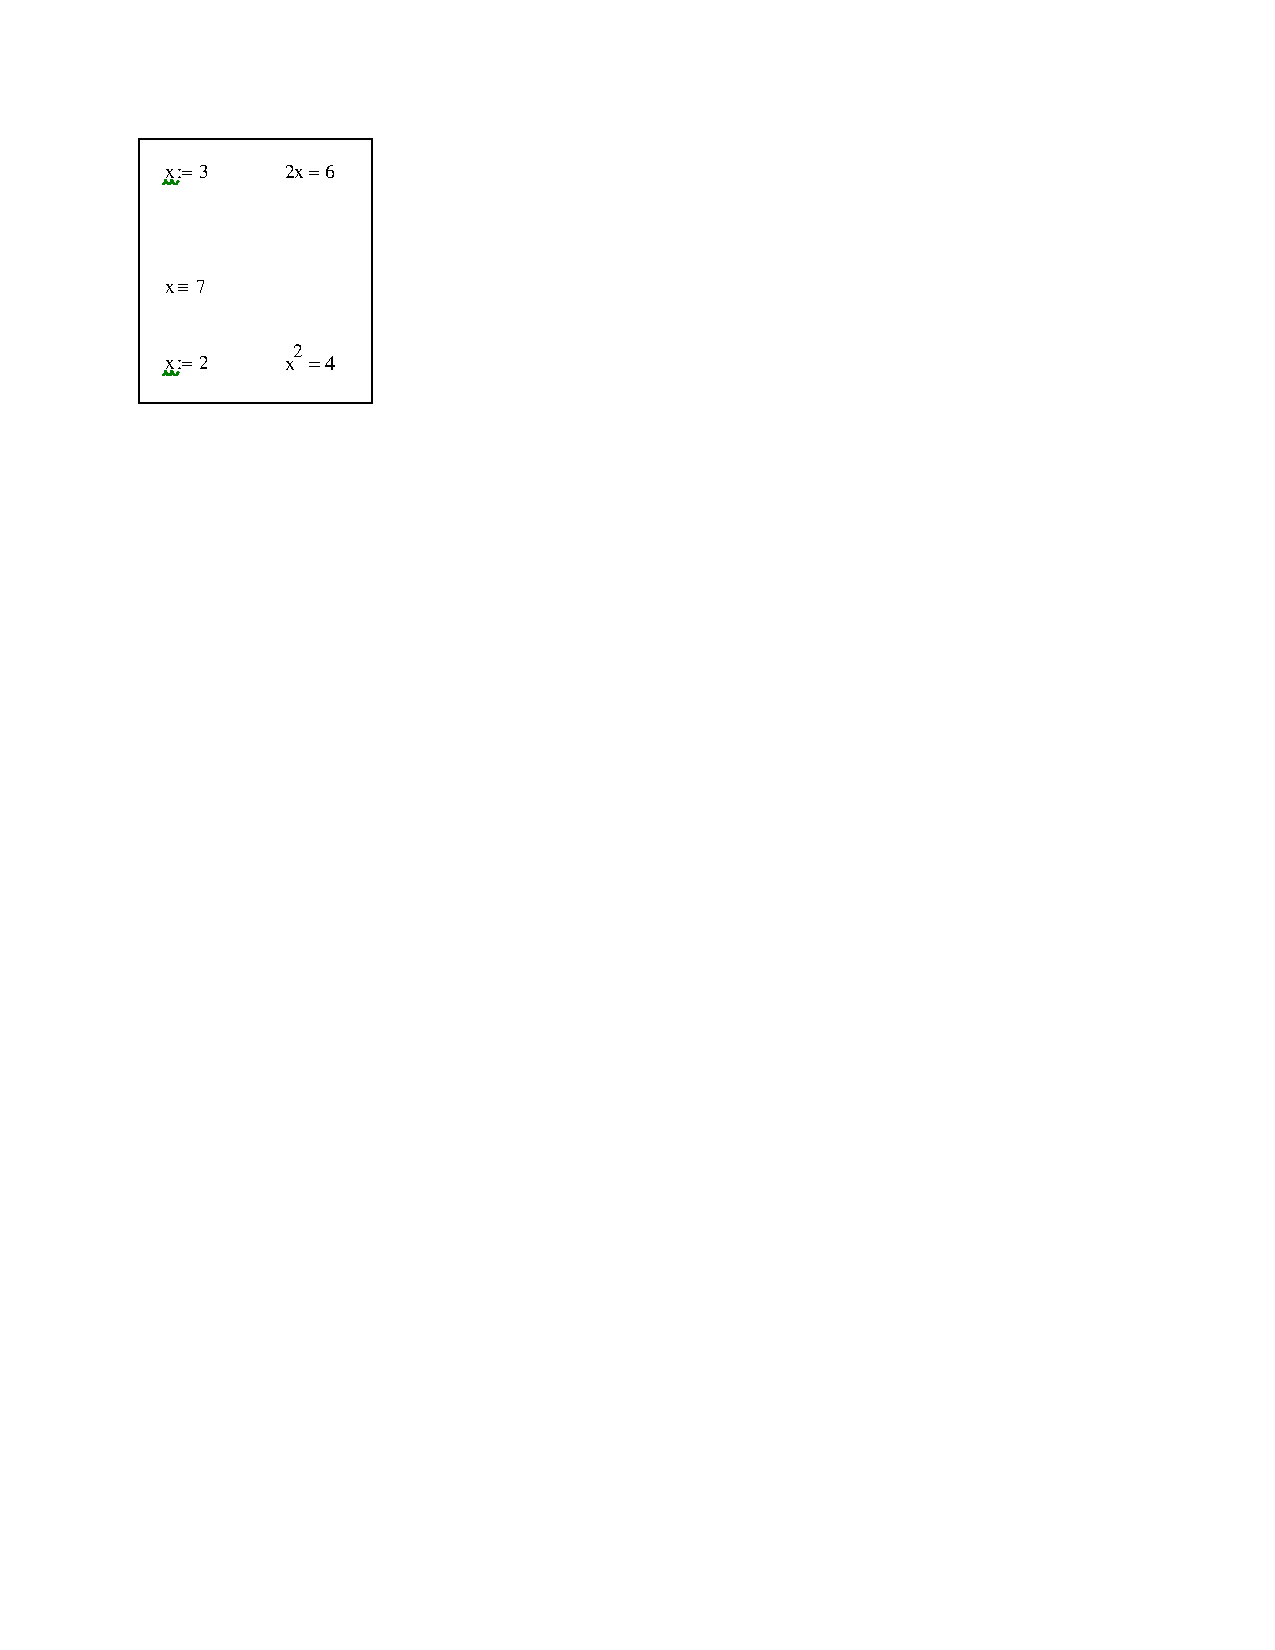
\includegraphics[bb=1in 8in 3in 10.2in]{figures/mathcad_global_definition2.pdf} %Mathcad copied to Word, saved as pdf, guess bounding box size
%\end{center}
\newpage
\printexercises{exercises/11_exercises}

%\begin{adjustwidth}{-60pt}{-60pt}
%\sffamily 
%\exinput{exercises/11_ex_04}
%\rmfamily
%\end{adjustwidth}
%\definition{def:lineintegral}{\textbf{TITLE}}